% CSCI3753 - Operating Systems
% Spring 2013
% Programming Assignment 3
% By Stephen Bennett (3/28/13)

\documentclass[12pt]{article}

%\usepackage[text={6.5in, 9in}, centering]{geometry}
%\usepackage[top=1in,bottom=1in,right=1.0in,left=1.0in]{geometry}
\usepackage[margin=1.0in]{geometry}
\usepackage{graphicx}
\usepackage{url}        % \url{}
\usepackage{amsfonts}   % \mathbb
\usepackage{float}      % H figure placement specifier
\usepackage{listings}   % Input code from file directly
\usepackage{xcolor}     % Allow colored code
\usepackage[section]{placeins}  % Defines \FloatBarrier and optionally redefines \section to include \FloatBarrier
\usepackage{subcaption} % Allows subfigures

\title{Programming Assignment 3:\\Investigating the Linux Scheduler}
\author{
  Stephen Bennett\\
  CSCI 3753 - Operating Systems\\
  University of Colorado at Boulder\\
  Spring 2013\\
}
\date{\emph{Due Date: Sunday, March 31, 2013 11:55pm}}

\begin{document}

%%%%% Begin Title Page %%%%%
\maketitle

%%%%% Begin Abstract (Vertically Centered) %%%%%
\clearpage
\vspace*{\fill}
\begin{abstract}

The purpose of this project was to investigate the differences among the various Linux scheduling policies.  The scheduler was tested by gathering timing and execution information from three benchmark programs written to represent the three types of processes: compute bound, I/O bound, and a mix of the two.  It was determined that the ideal scheduling algorithm differs based on the type of process being scheduled.  Compute bound processes perform best under the SCHED\_OTHER scheduling policy, I/O bound processes perform best under a real-time scheduling policy, and mixed processes perform nearly equally under all scheduling policies.

\end{abstract}

\vspace*{\fill}

%%%%% Begin Main Sections %%%%%
\clearpage
\section{Introduction}

The purpose of this investigation into the Linux scheduler is to discover and discuss the differences among the various scheduling algorithms.  To do this, I will write three test programs \texttt{pi.c}, \texttt{rw.c} and \texttt{mix.c}, each representative of a different type of real world program.  The test system will then be loaded with multiple instances of these programs in order to produce various levels of system utilization.  The processes will be scheduled using specified scheduling policies.  Using the Linux \texttt{time} command, information about the run-time and execution of the benchmarks will be gathered.  All tests will be run on a desktop computer running 64-bit Linux Mint 14 Nadia with version
3.5.0-26-generic of the Linux kernel.


\section{Method}

\subsection{Benchmarks}

Three benchmarks were written, each testing one of the three possible program types: CPU bound, I/O bound, and a mix of the two.  In creating the CPU bound benchmark \texttt{pi.c}, some computationally intensive algorithm had to be chosen such that no time would be spent waiting on I/O operations or blocked on any other resource.  As a result of these constraints, the statistical algorithm for calculating the value of pi based on the Monte Carlo method was chosen\cite{Sayler-pi}.  This algorithm is relatively slow and very CPU intensive.  It creates an imaginary quarter circle of radius RAND\_MAX, generates a random pair (x,y) of coordinates $\{x,y \in \mathbb{R}\ |\ 0 \le x,y \le RAND\_MAX\}$, then calculates whether the (x,y) coordinate is within the quarter circle.  Additionally, there are two counters: one that keeps track of the total number of iterations and another that keeps track of the number of times the random (x,y) coordinate is found to be within the quarter circle.  Finally, once all iterations are complete, all that must be done is to calculate the probability of being in the quarter circle by dividing the two counters (inside circle divided by number of iterations) and multiplying the result by 4 to create a full circle rather than a quarter circle.

The I/O bound benchmark \texttt{rw.c} was written in such a way as to ``minimize the effects of filesystem buffering and maximize I/O delays''\cite{Sayler-PDF}.  In order to do this, the low level-level \texttt{read()} and \texttt{write()} system calls were used in conjunction with files opened in O\_SYNC mode.  O\_SYNC causes \texttt{write()} operations to block until the data is physically written to the disk rather than until the data is simply copied to a kernel buffer\cite{man-open}.  An input file and an output file are given to the program which then reads blocks of data from the input file and writes said data to the output file.  This process occurs multiple times with minimal CPU involvement, thus creating the I/O bound benchmark.  There is only a small amount of CPU use involved, primarily in setting up the input/output files and verifying the passed parameters.

The third and final benchmark program was the mixed benchmark  \texttt{mix.c}.  I wrote this benchmark as a combination of the ideas from the previous two benchmarks.  The program performs the same computation as the CPU bound process statistically calculating the value of pi, but every so many iterations it writes the current values of the counters and the estimated value of pi to a file.  This \texttt{write()} operation once again uses O\_SYNC mode to maximize I/O delays.

For each benchmark, I wrote a separate program (e.g. \texttt{rw-sched.c} for I/O benchmark, etc.) that took care of setting the correct scheduling policy and \texttt{fork()}ing the desired number of child processes.  Each time a process needs to read from or write to a file, it needs its own input or output file in order to prevent additional waiting due to mutual exclusions and not actual I/O as is desired; the housekeeping programs ensure that each process has its own unique input/output file.

\subsection{Testing and Data}

I wrote a Bash script to take care of automation for running the 27 different test cases.  Each test case was run three times and the results were averaged in order to get more accurate data.  While compiling the source code with the Makefile, a single 1 MB file called \texttt{rwinput} is created.  It is created by reading 1024 blocks of size 1024 kB of random data from \texttt{/dev/urandom} and writing the data to \texttt{rwinput}.  To ensure that each instance of the I/O bound benchmark program had its own input file, the Bash script then copies \texttt{rwinput} as many times as necessary and gives each copy a unique name.  The \texttt{rw-sched.c} program then passes the proper unique input file name to each child process \texttt{fork()}ed.  Through the use of the \texttt{time} command and nested \texttt{for} loops iterating over both the number of child processes to \texttt{fork()} and the scheduling algorithms, I gathered results for each of the test cases.  From the \texttt{time} command I gathered the following aggregate information for each set of processes:
\begin{itemize}
  \item Wall time (turnaround time) - the real time the process took to complete from when it entered the system to when it completed
  \item User time - the amount of CPU-seconds the process spent executing in user mode
  \item System time - the amount of CPU-seconds the process spent executing in kernel mode
  \item The percentage of the CPU that the process got
  \item The number of times the process was context switched
  \item The number of times the process was blocked on I/O
\end{itemize}

\subsection{Test System}

All of the tests were run on a desktop running 64-bit Linux Mint 14 Nadia with version \texttt{3.5.0-26-generic} of the Linux kernel.  This all runs on a quad-core Intel Core i5-2500K CPU running at 3.30GHz with 8GB of RAM.  Each core is capable of executing a single hardware thread; thus four processes may be running concurrently in this system.  The primary disk for the system is a 1TB 7200 RPM Western Digital with 32MB of cache which uses the SATA II interface.  All of the programs were compiled using \texttt{GNU C Compiler version 4.7.2 (Ubuntu/Linaro 4.7.2-2ubuntu1)}.  The time slice for the Round Robin scheduling algorithm for this setup is 0.1000006 seconds.


\section{Results}

%\newcommand{\newfigure}[2][0.8]{
  %\begin{figure}[hbtp]
    %\centering
    %\includegraphics[scale=#1]{img/#2.eps}
    %\caption{}
    %\label{fig:#2}
  %\end{figure}
%}

Using the methodology described above, I gathered the following results. Figure~\ref{fig:cpu-wall-child} on page~\pageref{fig:cpu-wall-child}, Figure~\ref{fig:io-wall-child} on page~\pageref{fig:io-wall-child}, and Figure~\ref{fig:mix-wall-child} on page~\pageref{fig:mix-wall-child} show the average wall time per child process averaged over three trial runs for the three different benchmarks.  Each figure shows the results for a specific benchmark and compares the performance of each scheduling policy based on number of child processes.

The CPU bound benchmark results in Figure~\ref{fig:cpu-wall-child} show that while the number of processes remains relatively low the SCHED\_OTHER scheduling policy out-paces the other policies tested; at high numbers of processes the advantage disappears for all intents and purposes.  Both of the Real-time scheduling algorithms perform relatively equally regardless of number of processes.  Additionally, as the number of processes increases, each process takes more time to complete.

\begin{figure}[H]
  \centering
  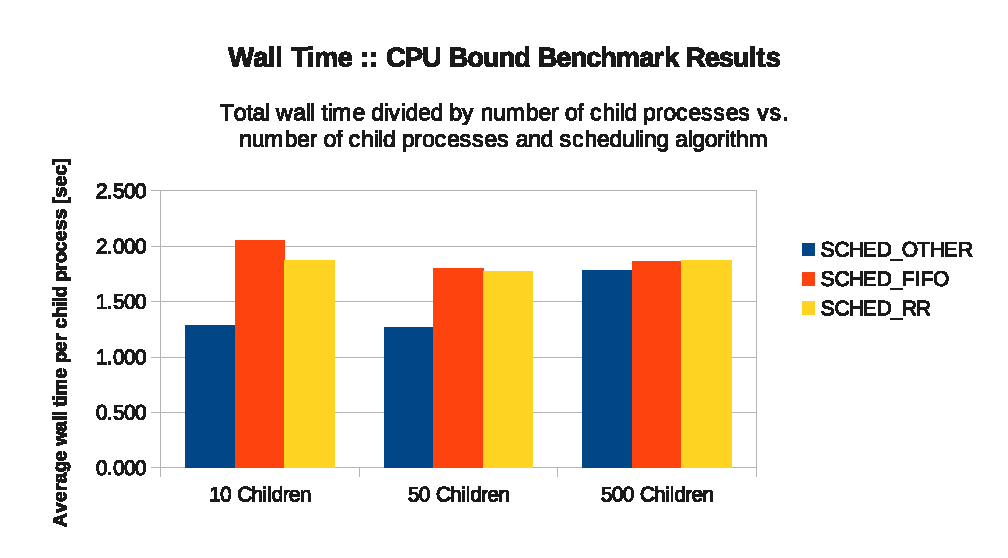
\includegraphics[scale=0.8]{img/cpu-wall-child.eps}
  \caption{}
  \label{fig:cpu-wall-child}
\end{figure}

The I/O bound benchmark results in Figure~\ref{fig:io-wall-child} show that a higher priority scheduling algorithm improves wall time.  As the number of processes increases, the performance of the different scheduling algorithms converges and the amount of time for each process to complete decreases.

\begin{figure}[H]
  \centering
  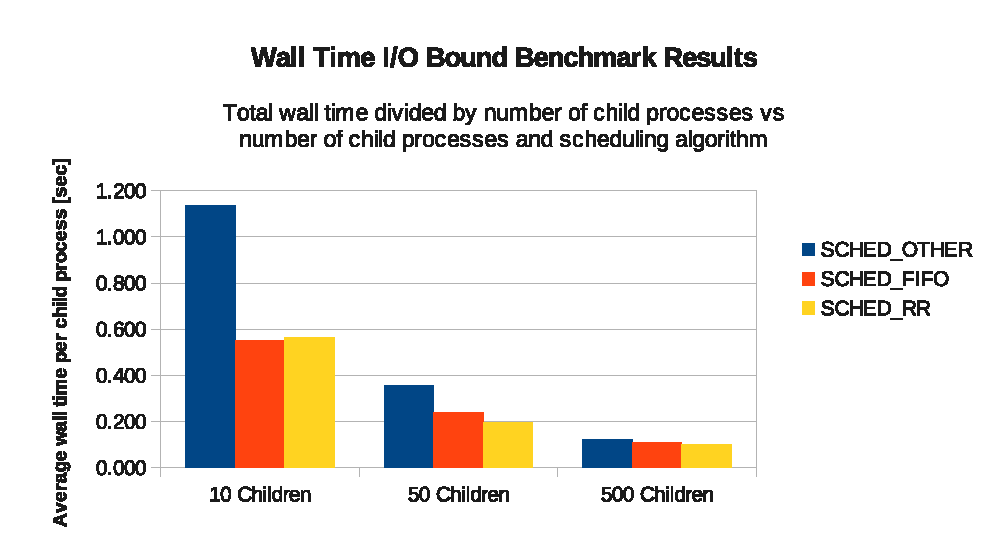
\includegraphics[scale=0.8]{img/io-wall-child.eps}
  \caption{}
  \label{fig:io-wall-child}
\end{figure}

The mixed benchmark results in Figure~\ref{fig:mix-wall-child} show that the scheduling policy does not have a significant impact on the amount of time each process takes to complete execution.  As the number of processes increases, the amount of time each process takes to complete its execution decreases.

\begin{figure}[H]
  \centering
  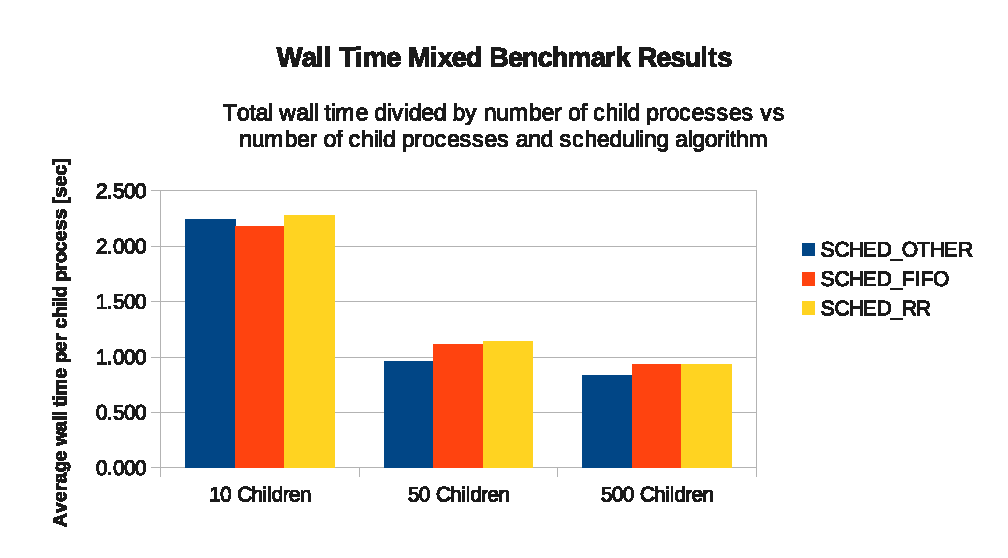
\includegraphics[scale=0.8]{img/mix-wall-child.eps}
  \caption{}
  \label{fig:mix-wall-child}
\end{figure}

Figure~\ref{fig:cpu-cs-child} on page~\pageref{fig:cpu-cs-child} and Figure~\ref{fig:mix-cs-child} on page~\pageref{fig:mix-cs-child} show that the number of times a process is context switched under a Real-time scheduling policy remains constant as the number of processes increases.  On the other hand, with the SCHED\_OTHER scheduling policy as the number of child processes increases, so does the amount of context switches per process.

\begin{figure}[H]
  \centering
  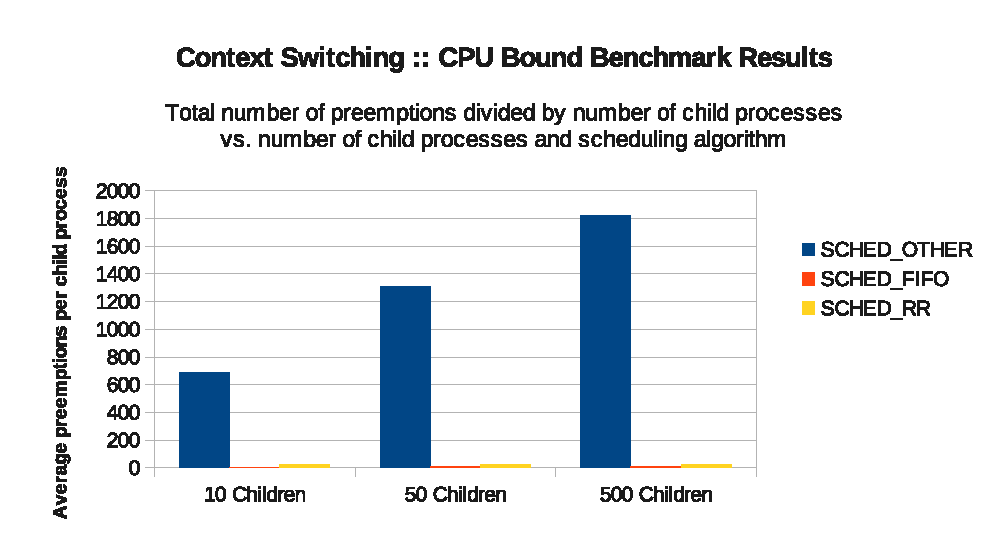
\includegraphics[scale=0.8]{img/cpu-cs-child.eps}
  \caption{}
  \label{fig:cpu-cs-child}
\end{figure}

\begin{figure}[H]
  \centering
  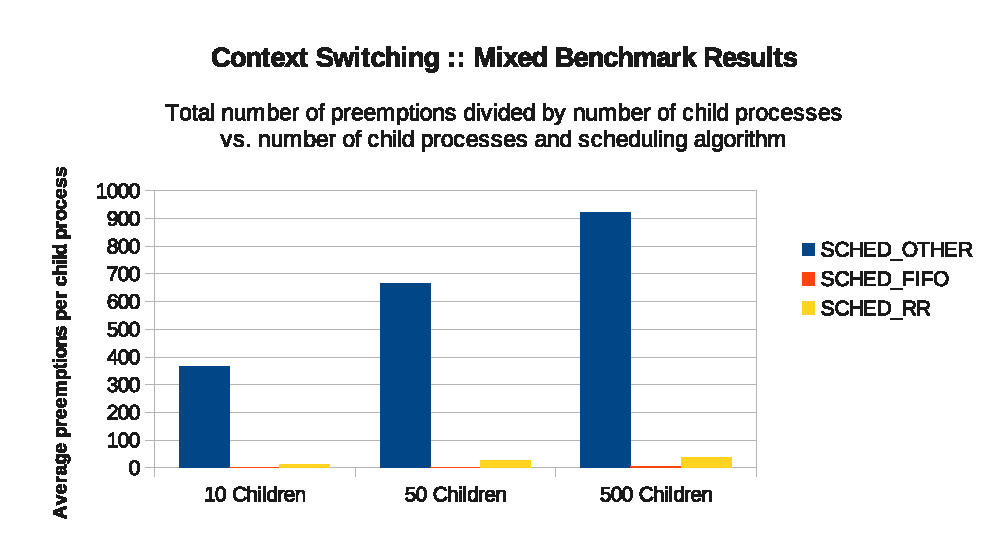
\includegraphics[scale=0.8]{img/mix-cs-child.eps}
  \caption{}
  \label{fig:mix-cs-child}
\end{figure}

As can be seen in Figure~\ref{fig:cpu-thruput-child} on page \pageref{fig:cpu-thruput-child} showing the throughput of the CPU bound benchmark, the highest throughput is achieved using the SCHED\_OTHER scheduling algorithm at relatively low quantities of child processes.  As the number of processes increases, all of the scheduling algorithms converge on a throughput of roughly one process completed every two seconds.

%\begin{figure}[H]
  %\centering
  %\begin{subfigure}[b]{0.495\textwidth}
    %\centering
    %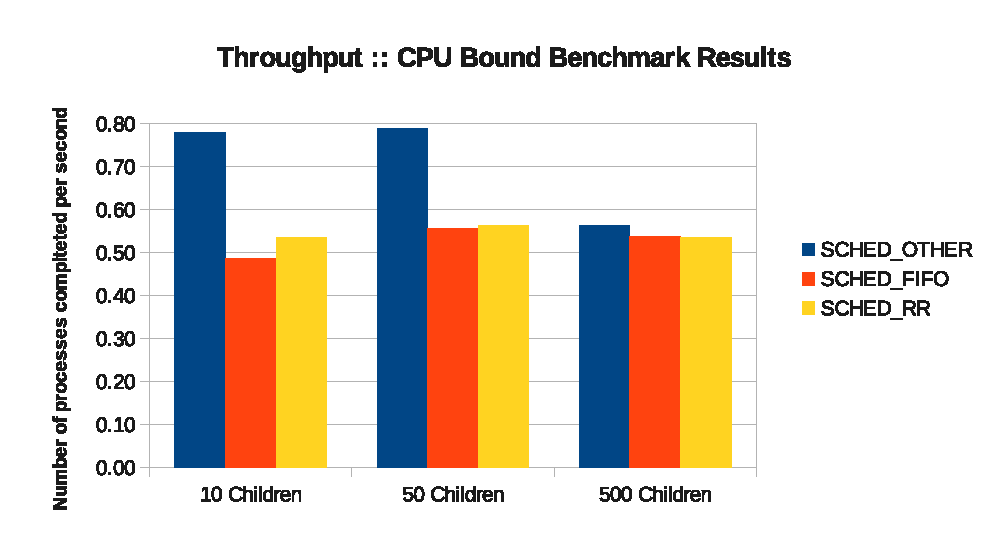
\includegraphics[scale=0.5]{img/cpu-thruput-child.eps}
    %\caption{}
    %\label{fig:cpu-thruput-child}
  %\end{subfigure}
  %% ~ % Non-breaking space
  %\begin{subfigure}[b]{0.495\textwidth}
    %\centering
    %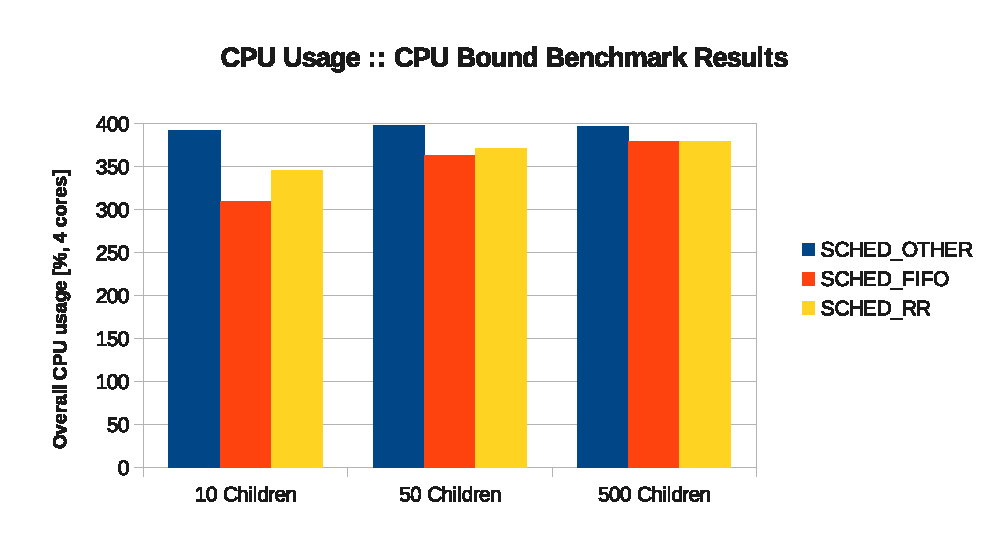
\includegraphics[scale=0.5]{img/cpu-usage-child.eps}
    %\caption{}
    %\label{fig:cpu-usage-child}
  %\end{subfigure}
%\end{figure}

\begin{figure}[H]
  \centering
  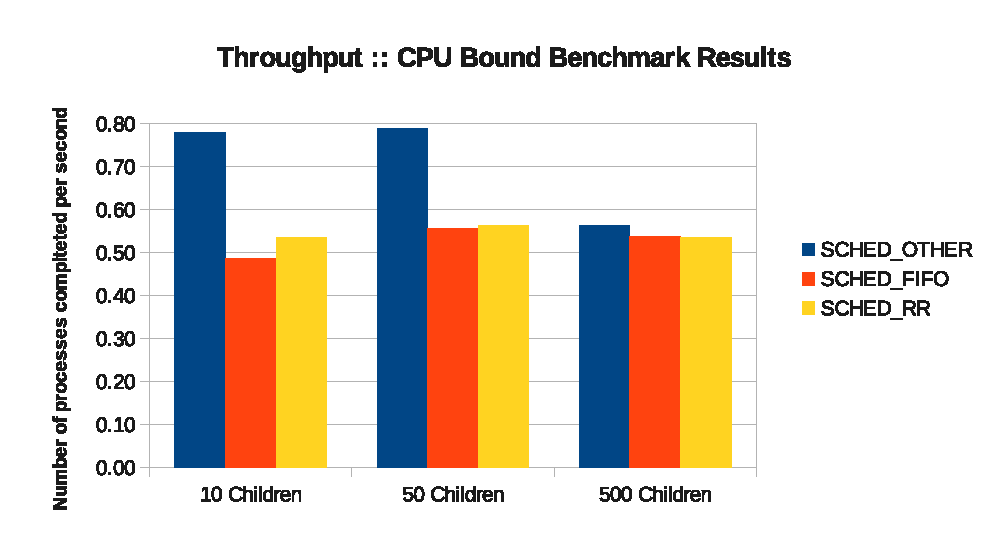
\includegraphics[scale=0.8]{img/cpu-thruput-child.eps}
  \caption{}
  \label{fig:cpu-thruput-child}
\end{figure}

The throughput results in Figure~\ref{fig:io-thruput-child} on page~\pageref{fig:io-thruput-child} show that increasing the number of concurrently executing I/O bound processes increases the overall throughput of the system.  Additionally, the higher the priority of the scheduling algorithm, the higher the throughput.

\begin{figure}[H]
  \centering
  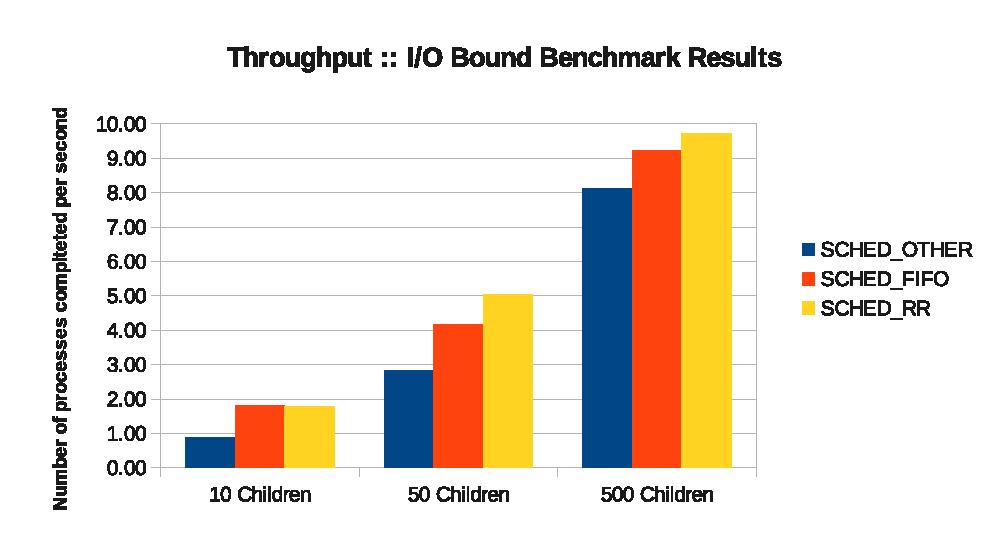
\includegraphics[scale=0.8]{img/io-thruput-child.eps}
  \caption{}
  \label{fig:io-thruput-child}
\end{figure}

The throughput results in Figure~\ref{fig:mix-thruput-child} on page~\pageref{fig:mix-thruput-child} show a similar overall positive correlation between number of processes and throughput to the I/O throughput results.  However, at higher numbers of processes, the SCHED\_OTHER scheduling algorithm seems to show a slight lead, similar to what is seen at lower numbers of running processes in Figure~\ref{fig:cpu-thruput-child} on page~\pageref{fig:cpu-thruput-child}.

\begin{figure}[H]
  \centering
  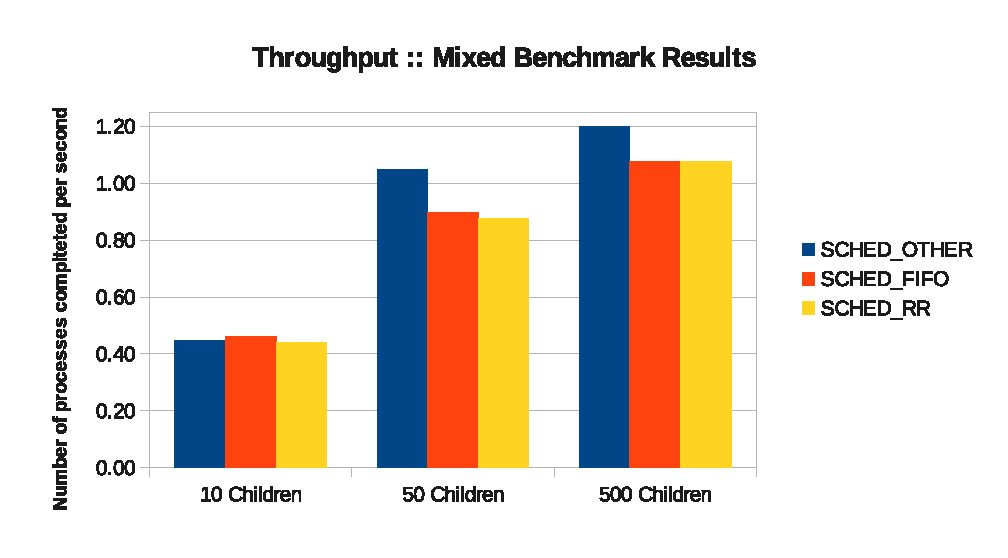
\includegraphics[scale=0.8]{img/mix-thruput-child.eps}
  \caption{}
  \label{fig:mix-thruput-child}
\end{figure}


\section{Analysis}

Negative correlation wall time could be attributed to higher parallelism between CPU and I/O.


\section{Conclusion}

The purpose of this investigation into the Linux Scheduler was to determine how each scheduling algorithm performed under various circumstances.  The real-time scheduling algorithms SCHED\_RR and SCHED\_FIFO proved to be best suited for processes that involved performing a lot of I/O operations.  SCHED\_RR performed the best or equally as well for I/O bound processes under all levels of system utilization.  For CPU bound processes, SCHED\_OTHER was clearly the optimal scheduling algorithm.  For low to medium levels of system utilization, the wall time was significantly less, and for high system utilization the wall time was still slightly lower.  Additionally, the SCHED\_OTHER scheduling algorithm was able to maximize throughput and CPU usage.  Lastly, for mixed processes that involved both computationally and I/O intensive sections there proved to be no clear best scheduling policy.  The results support SCHED\_OTHER slightly more than SCHED\_FIFO and least of all SCHED\_RR.  These results lend themselves to the theory that the mixed benchmark was written to be more CPU bound than I/O bound.


\clearpage
% The second parameter dictates how many digits to use for references
\begin{thebibliography}{9}      % Allows up to 9 references
%\begin{thebibliography}{56}     % Allows up to 99 references

\bibitem{Jones-InsideCFS} Jones, M. Tim.
  \newblock \emph{Inside the Linux 2.6 Completely Fair Scheduler}.
  \newblock IBM developerWorks: 2009.
  \newblock Accessed 06/01/12.
  \newblock \url{http://www.ibm.com/developerworks/linux/library/l-completely-fair-scheduler/}.

\bibitem{K&R} Kernighan, Brian and Dennis, Ritchie.
  \newblock \emph{The C Programming Language}.
  \newblock Second Edition: 2009.
  \newblock Prentice Hall: New Jersey.

\bibitem{Kolivas-BFS} Kolivas, Con.
  \newblock \emph{BFS - The Brain Fuck Scheduler}.
  \newblock 2009.
  \newblock Accessed 06/01/12.
  \newblock \url{http://ck.kolivas.org/patches/bfs/sched-BFS.txt}.

\bibitem{Kolivas-BFSFAQ} Kolivas, Con.
  \newblock \emph{FAQS about BFS}.
  \newblock v0.330: 2009.
  \newblock Accessed 06/01/12.
  \newblock \url{http://ck.kolivas.org/patches/bfs/bfs-faq.txt}.

\bibitem{Kumar-MultiCFS} Kumar, Avinesh.
  \newblock \emph{Multiprocessing with the Completely Fair Scheduler}.
  \newblock IBM developerWorks: 2008.
  \newblock Accessed 06/01/12.
  \newblock \url{http://www.ibm.com/developerworks/linux/library/l-cfs/}.

\bibitem{Le-StudyLKS} Le, Thang Minh.
  \newblock \emph{A Study on Linux Kernel Scheduler: version 2.6.32}.
  \newblock 2009.
  \newblock Accessed 06/01/12.
  \newblock \url{http://www.scribd.com/thangmle/d/24111564-Project-Linux-Scheduler-2-6-32}.

\bibitem{Molnar-CFS} Molnar, Ingo.
  \newblock \emph{This is the CFS scheduler}.
  \newblock 2007.
  \newblock Accessed 06/01/12.
  \newblock \url{http://people.redhat.com/mingo/cfs-scheduler/sched-design-CFS.txt}.

\bibitem{tubes} Stevens, Ted.
  \newblock \emph{Speech on Net Neutrality Bill}.
  \newblock 2006.
  \newblock \url{http://youtu.be/f99PcP0aFNE}.

\bibitem{StrunkWhite} Strunk, William, Jr. and White, E.B.
  \newblock \emph{The Elements of Style}.
  \newblock Fourth Edition: 2000.
  \newblock Pearson: New York.

\end{thebibliography}


%%%%% Begin Appendices %%%%%
\appendix

\clearpage
\section{Appendix - Raw Data}



\clearpage
\newgeometry{top=1in,bottom=1in,right=0.5in,left=0.5in}
%\section{Appendix - All Code}

\lstdefinestyle{customc}{
 belowcaptionskip=1\baselineskip,
 breaklines=true,
 frame=L,
 xleftmargin=\parindent,
 language=C,
 showstringspaces=false,
 basicstyle=\footnotesize\ttfamily,
 keywordstyle=\bfseries\color{green!40!black},
 commentstyle=\itshape\color{purple!40!black},
 identifierstyle=\color{blue},
 stringstyle=\color{orange},
 escapechar=@,
}
\lstdefinestyle{custommake}{
 belowcaptionskip=1\baselineskip,
 breaklines=true,
 frame=L,
 xleftmargin=\parindent,
 language=make,
 showstringspaces=false,
 basicstyle=\footnotesize\ttfamily,
 keywordstyle=\bfseries\color{green!40!black},
 commentstyle=\itshape\color{purple!40!black},
 identifierstyle=\color{blue},
 stringstyle=\color{orange},
}
%\lstset{escapechar=@,style=customc}

\newcommand{\includecode}[2]{\lstinputlisting[style=customc, caption=#1 \texttt{#2.c}, label=lst:#2]{../#2.c}}

\includecode{CPU Bound Benchmark}{pi}
\includecode{CPU Bound Benchmark Scheduler}{pi-sched}
\includecode{I/O Bound Benchmark}{rw}
\includecode{I/O Bound Benchmark Scheduler}{rw-sched}
\includecode{Mixed Benchmark}{mix}
\includecode{Mixed Benchmark Scheduler}{mix-sched}
\lstinputlisting[style=custommake, caption=Makefile, label=lst:makefile]{../Makefile}

\restoregeometry

\end{document}
